\documentclass[a4paper,11pt]{beamer}
\usepackage{etex}
\usepackage{lmodern}
\usepackage[french]{babel}
\usepackage[T1]{fontenc}
\usepackage[utf8]{inputenc}
% \usepackage{listings}
\usepackage{graphicx} 
\usepackage{ragged2e} 
\usepackage{enumitem}
\usepackage{array}
% \usepackage{tikz} 
% \usepackage{pgf-umlcd} 
\usepackage{csquotes}
\usepackage{pst-sigsys}
\usepackage{amsmath,amsfonts,bm}
\usepackage{pstricks-add}
% \usepackage{physics}
% \usepackage{ulem}
% \usepackage{wasysym}
% \usepackage{hyperref}
% \usepackage{color}


\setenumerate{label*=\arabic*.} 

\setbeamertemplate{navigation symbols}{}  
  
\usetheme{Darmstadt} 
\setbeamertemplate{footline}{\insertframenumber/\inserttotalframenumber}
\title{L3 - CMI017 : Signaux et Systèmes\\Séquence III}
\author{BULOUP Frank}
\institute{Aix Marseille Université\\Institut des Sciences du Mouvement}
\date{}

\setbeamertemplate{footline} 
{  
	\begin{beamercolorbox}[ht=2.5ex,dp=1.125ex,%
      leftskip=.3cm,rightskip=.3cm plus1fil]{title in head/foot}%
      {\usebeamerfont{title in head/foot}\insertshorttitle} \hfill    
      \insertframenumber / \inserttotalframenumber%
    \end{beamercolorbox}%
%     \begin{beamercolorbox}[colsep=1.5pt]{lower separation line foot}
%     \end{beamercolorbox} 
}

\newcounter{exampleBlockCounter}
\setcounter{exampleBlockCounter}{1}

\definecolor{comment}{rgb}{0.12, 0.38, 0.18 } %adjusted, in Eclipse: {0.25, 0.42, 0.30 } = #3F6A4D
\definecolor{keyword}{rgb}{0.37, 0.08, 0.25}  % #5F1441
\definecolor{string}{rgb}{0.06, 0.10, 0.98} % #101AF9
\definecolor{myGreen}{rgb}{0,0.4,0}

% \lstset {language=Java,
%  frame=single,
%  frameround=tttt,
%  rulesepcolor=\color{black},
%  showspaces=false,showtabs=false,tabsize=2,
%  numberstyle=\tiny,numbers=left,
%  stringstyle=\color{string},
%  keywordstyle = \color{keyword}\bfseries,
%  commentstyle=\color{comment}\itshape,
%  basicstyle=\ttfamily\footnotesize,
%  breaklines=true,
%  captionpos=b
% }

% \renewenvironment{package}[2][\umlcdPackageTitle]{
% \edef\umlcdPackageTitle{#2}
% \def\umlcdPackageFit{}
% \def\umlcdPackageName{#1}
% }{
%   \begin{pgfonlayer}{background}
%   \node[umlcd style, draw, inner sep=0.5cm, fit = \umlcdPackageFit] (\umlcdPackageName) {};
%   \node[umlcd style, draw, outer ysep=-0.5, anchor=south west] (\umlcdPackageName caption) at
%   (\umlcdPackageName.north west) {\umlcdPackageTitle};
%   \end{pgfonlayer}
% }

\begin{document}

\begin{frame}[plain]  
	\titlepage  
	\center{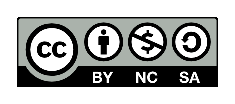
\includegraphics[scale=0.75]{images/by-nc-sa.eps}}
	\vspace{1cm}
	
	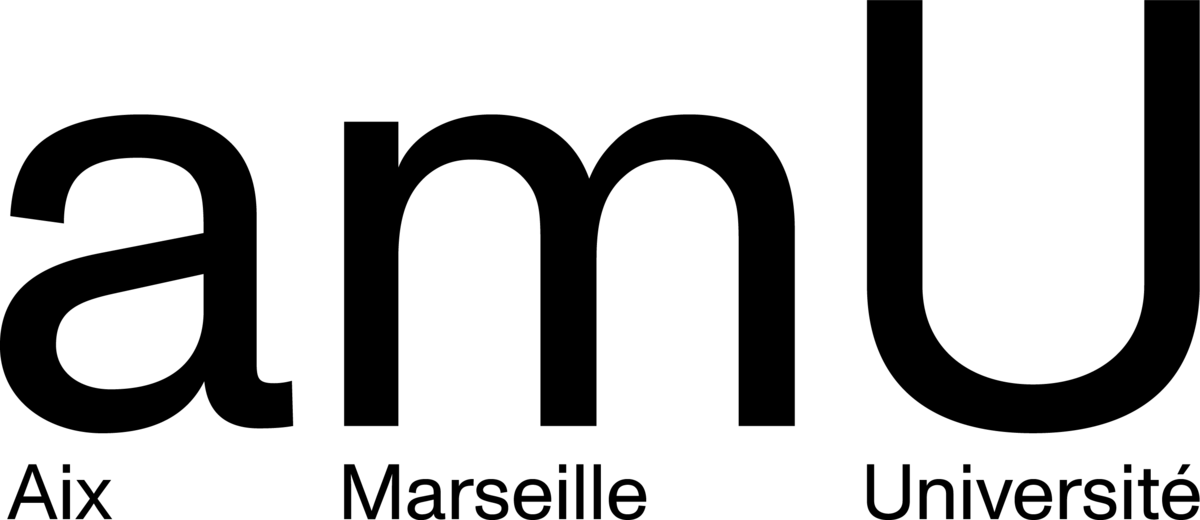
\includegraphics[scale=0.6]{images/LogoAMU.png}\hspace*{2cm}
	
\includegraphics[scale=0.2]{images/LogoCNRS.eps}\hspace*{2cm}
	
\includegraphics[scale=0.1]{images/LogoISM.eps}
\end{frame} 
  

\begin{frame}{Plan de cette séquence}
	\tableofcontents[hideallsubsections]
\end{frame}

\AtBeginSection[]{
\begin{frame}{Signaux et Systèmes}
	\tableofcontents[currentsection,hideallsubsections]
\end{frame}
}

\section{Fonction de transfert en $\mathcal{R}$} 
\subsection{Généralités}  

\begin{frame}
\begin{block}{Équation aux différences de $S_1$}
\[
s(n) = \frac{e(n) + e(n-1)}{2}
\]
\end{block}
\begin{block}{Diagramme bloc de $S_1$}
\begin{figure}
	\begin{pspicture}[showgrid=false](0,0)(7,2)
		\psset{arrows=->}
		\pssignal(0.5,1.5){e}{e(n)}
		\pssignal(6.5,1.5){s}{s(n)}
		\psfblock[framesize=1.5 0.75](2.75,0.5){delay}{Retard}
		\pscircleop(4,1.5){add}
		\pscircleop[operation=times](5,1.5){times}
		\rput(5,1){$\frac{1}{2}$}
		\dotnode(1.5,1.5){node}
		\ncline{e}{add}
		\ncline{add}{times}
		\ncline{times}{s}
		\ncangle[angleA = 0, angleB = -90]{->}{delay}{add}
		\ncangle[angleA = -90, angleB = 180]{->}{node}{delay}
	\end{pspicture}
\end{figure}
\end{block}
\end{frame}

\begin{frame}
\centering
\textbf{\textcolor{red}{Pensez maintenant en terme de signal et pas
d'échantillon}}
\vspace{0.5cm}

\begin{itemize}
	\justifying
  \item Les noeuds des diagrammes blocs représent les signaux, l'ensemble des
	échantillons
  \item Les opérateurs agissent sur le signal et pas uniquement sur un
  seul de ses échantillons
\end{itemize}
\pause
\begin{block}{Diagramme bloc de $S_1$}
\begin{figure}
	\begin{pspicture}[showgrid=false](0,0)(7,2)
		\psset{arrows=->}
		\pssignal(0.5,1.5){e}{E}
		\pssignal(6.5,1.5){s}{S}
		\psfblock[framesize=1.5 0.75](2.75,0.5){delay}{Retard}
		\pscircleop(4,1.5){add}
		\pscircleop[operation=times](5,1.5){times}
		\rput(5,1){$\frac{1}{2}$}
		\dotnode(1.5,1.5){node}
		\ncline{e}{add}
		\ncline{add}{times}
		\ncline{times}{s}
		\ncangle[angleA = 0, angleB = -90]{->}{delay}{add}
		\ncangle[angleA = -90, angleB = 180]{->}{node}{delay}
	\end{pspicture}
\end{figure}
\end{block}
\centering
\textbf{\textcolor{red}{E et S sont des « vecteurs » d'échantillons}}
\end{frame}

\begin{frame}
\begin{block}{Diagramme bloc de $S_1$}
\begin{figure}
	\begin{pspicture}[showgrid=false](0,0)(7,2)
		\psset{arrows=->}
		\pssignal(0.5,1.5){e}{E}
		\pssignal(6.5,1.5){s}{S}
		\psfblock[framesize=1.5 0.75](2.75,0.5){delay}{$\mathcal{R}$}
		\pscircleop(4,1.5){add}
		\pscircleop[operation=times](5,1.5){times}
		\rput(5,1){$\frac{1}{2}$}
		\dotnode(1.5,1.5){node}
		\ncline{e}{add}
		\ncline{add}{times}
		\ncline{times}{s}
		\ncangle[angleA = 0, angleB = -90]{->}{delay}{add}
		\ncangle[angleA = -90, angleB = 180]{->}{node}{delay}
	\end{pspicture}
\end{figure}
\end{block}
\centering
\textbf{\textcolor{red}{L'opérateur de \textbf{Retard} se
traduit alors comme un décalage vers la droite, noté \textbf{$\mathcal{R}$
pour « right shift »}}}
\end{frame}

\begin{frame}
\begin{block}{Notation}
\centering
$\mathcal{R}$ : opérateur de décalage vers la droite (retard d'un échantillon)
\vspace{0.5cm}

On note : $S = \mathcal{R}\{E\} = \mathcal{R}E$\\
\vspace{0.5cm}

$S$ et $E$ représentent les signaux $s(n)$ et $e(n)$ pour l'ensemble de
leurs échantillons
\end{block}
\pause
\begin{block}{Conséquence}
\centering
\textbf{\textcolor{red}{On peut écrire simplement, à partir du diagramme bloc
ou de l'équation aux différences, une relation entrée/sortie polynomiale en
$\mathcal{R}$}}
\end{block}
\end{frame}

\begin{frame}
\begin{block}{Équation aux différences de $S_1$}
\[
s(n) = \frac{e(n) + e(n-1)}{2}
\]
\end{block}
\begin{block}{Diagramme bloc de $S_1$}
\begin{figure}
	\begin{pspicture}[showgrid=false](0,0)(7,2)
		\psset{arrows=->}
		\pssignal(0.5,1.5){e}{e(n)}
		\pssignal(6.5,1.5){s}{s(n)}
		\psfblock[framesize=1.5 0.75](2.75,0.5){delay}{$\mathcal{R}$}
		\pscircleop(4,1.5){add}
		\pscircleop[operation=times](5,1.5){times}
		\rput(5,1){$\frac{1}{2}$}
		\dotnode(1.5,1.5){node}
		\ncline{e}{add}
		\ncline{add}{times}
		\ncline{times}{s}
		\ncangle[angleA = 0, angleB = -90]{->}{delay}{add}
		\ncangle[angleA = -90, angleB = 180]{->}{node}{delay}
	\end{pspicture}
\end{figure}
\end{block}
\pause
\begin{block}{Notation en $\mathcal{R}$}
\[
S = \frac{E + \mathcal{R}E}{2} = \frac{1 + \mathcal{R}}{2} E\Leftrightarrow
\frac{S}{E} = \mathcal{H}_{1}(\mathcal{R}) = \frac{1 +
\mathcal{R}}{2}
\]
\end{block}
\end{frame}

\begin{frame}
\begin{exampleblock}{Exercice \Roman{exampleBlockCounter} - Utilisation de la
notation en $\mathcal{R}$}
\justifying
On met en cascade deux systèmes $S_1$. 
\begin{enumerate}
\justifying
\item Quelle est la notation en $\mathcal{R}$ de ce nouveau système $S_2$ à
partir :
\begin{enumerate}	
	\item de l'équation aux différences de $S_1$ ?
	\item du diagramme blocs de $S_1$ ?
	\item En déduire l'expression de $\mathcal{H}_{2}(\mathcal{R})$
\end{enumerate}
\item Quelle est la réponse impulsionnelle de ce nouveau système ? (utiliser
	  la fonction \textbf{impz} de Matlab sur une dixaine d'échantillons)
\end{enumerate}
\end{exampleblock}
\end{frame}

\begin{frame}
\begin{exampleblock}{Exercice \Roman{exampleBlockCounter} - À partir de l'équation aux différences}
\[
\begin{aligned}
	s_1(n) &= \frac{e(n) + e(n-1)}{2}\\
	s(n) &= \frac{s_1(n) + s_1(n-1)}{2}\\
	\pause
	s(n) &= \frac{\frac{e(n) + e(n-1)}{2} + \frac{e(n-1) + e(n-2)}{2}}{2}\\
	\pause
	s(n) &= \frac{e(n) + 2e(n-1) + e(n-2)}{4}\\
	\text{Finalement : }S &= \frac{1 + 2\mathcal{R} + \mathcal{R}^2}{4} E
\end{aligned}
\]
\end{exampleblock}
\end{frame}

\begin{frame}
\begin{exampleblock}{Exercice \Roman{exampleBlockCounter} - À partir du
diagramme blocs}
\begin{figure}
	\begin{pspicture}[showgrid=false](0,0)(10,2)
		\psset{arrows=->}
		\pssignal(0.5,1.5){e}{$E$}
		\pssignal(5,1.75){s1}{$S_1$}
		\pssignal(9.5,1.5){s}{$S$}
		\psfblock[framesize=1 0.75](2.5,0.5){delay}{$\mathcal{R}$}
		\pscircleop(3.5,1.5){add}
		\pscircleop[operation=times](4.5,1.5){times}
		\rput(4.5,1){$\frac{1}{2}$}
		\dotnode(1.5,1.5){node}
		\ncline{e}{add}
		\ncline{add}{times}
		\ncline{times}{add2}
		\ncangle[angleA = 0, angleB = -90]{->}{delay}{add}
		\ncangle[angleA = -90, angleB = 180]{->}{node}{delay}
		\psfblock[framesize=1 0.75](6,0.5){delay2}{$\mathcal{R}$}
		\pscircleop(7,1.5){add2}
		\pscircleop[operation=times](8,1.5){times2}
		\rput(8,1){$\frac{1}{2}$}
		\dotnode(5,1.5){node2}
		\ncline{times}{add2}
		\ncline{add2}{times2}
		\ncline{times2}{s}
		\ncangle[angleA = 0, angleB = -90]{->}{delay2}{add2}
		\ncangle[angleA = -90, angleB = 180]{->}{node2}{delay2}
	\end{pspicture}
\end{figure}
\[
\begin{aligned}
	S_1 &= \frac{1 + \mathcal{R}}{2}E\\
	S &= \frac{1 + \mathcal{R}}{2}S_1\\
	\pause
	S &= \frac{1 + \mathcal{R}}{2} \frac{1 + \mathcal{R}}{2} E\\
	\text{Finalement : }S &= \frac{1 + 2\mathcal{R} + \mathcal{R}^2}{4} E\\
	\text{ et }\mathcal{H}_{2}(\mathcal{R}) &= \frac{1 + 2\mathcal{R} +
	\mathcal{R}^2}{4}
\end{aligned}
\]
\end{exampleblock}
\end{frame}

\begin{frame}
\begin{exampleblock}{Exercice \Roman{exampleBlockCounter} - Réponse
impulsionnelle de $S_2$}
\begin{figure}
	\begin{pspicture}[showgrid=false](-1,-0.5)(5,1.5)
		\psaxeslabels(0,0)(-1,-0.5)(5,1.5){$n$}{$s(n)$}
		\psaxes{->}(0,0)(-1,-0.5)(5,1.5)
		\psstem(-1,1){0,0.25,0.5,0.25,0}
		\psldots(4,0.5)
	\end{pspicture}
\end{figure}
\end{exampleblock}
\end{frame}
\stepcounter{exampleBlockCounter}

\subsection{Lien notation en $\mathcal{R}$ et réponse impulsionnelle}
\begin{frame}
\begin{table}
	\begin{tabular}{| >{\centering\arraybackslash}m{2in} |
	>{\centering\arraybackslash}m{2in} |}\hline
    Fonction de Transfert en $\mathcal{R}$ & Réponse
    impulsionnelle\\ \hline 
    $\mathcal{H}_1 (\mathcal{R}) = \frac{1+\mathcal{R}}{2}$ &
    \begin{pspicture}[showgrid=false](-1,-0.5)(4,1.5)
    	\psaxeslabels(0,0)(-1,-0.5)(4,1.5){$n$}{$s(n)$}
    	\psaxes{->}(0,0)(-1,-0.5)(4,1.5) 
    	\psstem(-1,1){0,0.5,0.5,0,0}
		\psldots(4,0.5)
		\rput(0.25,0.5){$\frac{1}{2}$}
		\rput(1.25,0.5){$\frac{1}{2}$}
	\end{pspicture}\\ \hline
    $\mathcal{H}_2 (\mathcal{R}) = \frac{1 + 2\mathcal{R} +
    \mathcal{R}^2}{4}$ & \begin{pspicture}[showgrid=false](-1,-0.5)(4,1.5)
		\psaxeslabels(0,0)(-1,-0.5)(4,1.5){$n$}{$s(n)$}
		\psaxes{->}(0,0)(-1,-0.5)(4,1.5)
		\psstem(-1,1){0,0.25,0.5,0.25,0}
		\psldots(4,0.5)
		\rput(0.25,0.25){$\frac{1}{4}$}
		\rput(1.25,0.5){$\frac{1}{2}$}
		\rput(2.25,0.25){$\frac{1}{4}$}
	\end{pspicture}\\ \hline
  \end{tabular}
\end{table}
\centering
\textbf{\textcolor{red}{Quel est le lien entre fonction de transfert\\ en
$\mathcal{R}$ et réponse impulsionnelle?}}
\end{frame}

\begin{frame}
\begin{table}
	\begin{tabular}{| >{\centering\arraybackslash}m{2in} |
	>{\centering\arraybackslash}m{2in} |}
    \hline
    Fonction de Transfert en $\mathcal{R}$ & Réponse
    impulsionnelle\\[0ex] \hline 
    $\mathcal{H}_1 (\mathcal{R}) = \frac{1+\mathcal{R}}{2}$ &
    \begin{pspicture}[showgrid=false](-1,-0.5)(4,1.5)
    	\psaxeslabels(0,0)(-1,-0.5)(4,1.5){$n$}{$s(n)$}
    	\psaxes{->}(0,0)(-1,-0.5)(4,1.5) 
    	\psstem(-1,1){0,0.5,0.5,0,0}
		\psldots(4,0.5)
		\rput(0.25,0.5){$\frac{1}{2}$}
		\rput(1.25,0.5){$\frac{1}{2}$}
	\end{pspicture} \\[0ex] \hline
    $\mathcal{H}_2 (\mathcal{R}) = \frac{1 + 2\mathcal{R} + \mathcal{R}^2}{4}$ & 
    \begin{pspicture}[showgrid=false](-1,-0.5)(4,1.5)
		\psaxeslabels(0,0)(-1,-0.5)(4,1.5){$n$}{$s(n)$}
		\psaxes{->}(0,0)(-1,-0.5)(4,1.5)
		\psstem(-1,1){0,0.25,0.5,0.25,0}
		\psldots(4,0.5)
		\rput(0.25,0.25){$\frac{1}{4}$}
		\rput(1.25,0.5){$\frac{1}{2}$}
		\rput(2.25,0.25){$\frac{1}{4}$}
	\end{pspicture} \\[0ex] \hline
  \end{tabular}
\end{table}
\centering 
\textbf{\textcolor{red}{Les coefficients du polynôme en
$\mathcal{R}$ donnent la réponse impulsionnelle du système. Dans ces deux
exemples, la réponse impulsionnelle est finie.}}
\end{frame}

\begin{frame}
\begin{exampleblock}{Exercice \Roman{exampleBlockCounter} - Fonction de
transfert en $\mathcal{R}$ et réponse impulsionnelle}
Soit un système dont la fonction de transfert en $\mathcal{R}$ est la suivante :
$$
\frac{S}{E} = 1 + \mathcal{R} + \mathcal{R}^2 + \mathcal{R}^3 + \mathcal{R}^4 + \mathcal{R}^5 
$$
\begin{enumerate}
  \item Quelle est la réponse impulsionnelle de ce système ?
  \item Quelle est son équation aux différences ?
\end{enumerate}
\end{exampleblock}
\end{frame}
\stepcounter{exampleBlockCounter}

\subsection{Fonction de transfert en $\mathcal{R}$ et système bouclé}
\begin{frame}
\begin{block}{Considérons le système $S_3$ suivant :} 
\begin{figure}
\begin{pspicture}[showgrid=false](0,0)(6,2)
	\psset{arrows=->}
	\pssignal(0.5,1.5){e}{E}
	\pssignal(5.5,1.5){s}{S}
	\psfblock[framesize=1.5 0.75](2.75,0.5){delay}{$\mathcal{R}$}
	\pscircleop(1.5,1.5){add} 
	\dotnode(4,1.5){node}
	\ncline{e}{add}
	\ncline{add}{s}
	\ncangle[angleA = -90, angleB = 180]{<-}{add}{delay}
	\ncangle[angleA = -90, angleB = 0]{->}{node}{delay}
	\psline[linecolor=red]{-}(2,1.4)(3.7,1.4)
	\psline[linecolor=red]{-}(3.7,1.4)(3.7,1)
	\psline[linecolor=red]{-}(3.7,1)(2,1)
	\psline[linecolor=red]{->}(2,1)(2,1.4)
\end{pspicture}
\end{figure}
\centering
Ce système comporte une boucle de rétroaction, un « feedback »
\end{block} 
\begin{exampleblock}{Exercice \Roman{exampleBlockCounter} - Système bouclé}
\begin{enumerate}
  \item Exprimer la fonction de transfert en $\mathcal{R}$ de ce nouveau système
  \item En déduire sa réponse impulsionnelle
  \item Donner l'expression de son équation aux différences
\end{enumerate}
\end{exampleblock} 
\end{frame}

\begin{frame}
\begin{exampleblock}{Exercice \Roman{exampleBlockCounter} - Fonction de
transfert en $\mathcal{R}$}
\begin{figure}
\begin{pspicture}[showgrid=false](0,0)(6,2)
	\psset{arrows=->}
	\pssignal(0.5,1.5){e}{E}
	\pssignal(5.5,1.5){s}{S}
	\psfblock[framesize=1.5 0.75](2.75,0.5){delay}{$\mathcal{R}$}
	\pscircleop(1.5,1.5){add} 
	\dotnode(4,1.5){node}
	\ncline{e}{add}
	\ncline{add}{s}
	\ncangle[angleA = -90, angleB = 180]{<-}{add}{delay}
	\ncangle[angleA = -90, angleB = 0]{->}{node}{delay}
\end{pspicture}
\end{figure}
$$
\begin{aligned}
S &= \mathcal{R}S + E\\
(1-\mathcal{R})S &= E\\
\frac{S}{E} &= \frac{1}{1-\mathcal{R}}
\end{aligned}
$$
\end{exampleblock} 
\centering
\textbf{\textcolor{red}{Remarque ?}}
\end{frame}

\begin{frame}
\begin{exampleblock}{Exercice \Roman{exampleBlockCounter} - Fonction de
transfert en $\mathcal{R}$}
\begin{figure}
\begin{pspicture}[showgrid=false](0,0)(6,2)
	\psset{arrows=->}
	\pssignal(0.5,1.5){e}{E}
	\pssignal(5.5,1.5){s}{S}
	\psfblock[framesize=1.5 0.75](2.75,0.5){delay}{$\mathcal{R}$}
	\pscircleop(1.5,1.5){add} 
	\dotnode(4,1.5){node}
	\ncline{e}{add}
	\ncline{add}{s}
	\ncangle[angleA = -90, angleB = 180]{<-}{add}{delay}
	\ncangle[angleA = -90, angleB = 0]{->}{node}{delay}
\end{pspicture}
\end{figure}
$$
\begin{aligned}
S &= \mathcal{R}S + E\\
(1-\mathcal{R})S &= E\\
\frac{S}{E} &= \frac{1}{1-\mathcal{R}}
\end{aligned}
$$
\end{exampleblock} 
\centering
\textbf{\textcolor{red}{Ce n'est pas un polynôme en $\mathcal{R}$\\ mais une
fonction rationnelle !\\
\pause
Il est donc impossible d'en déduire\\ directement la réponse impulsionnelle}}
\end{frame}

\begin{frame}
\begin{exampleblock}{Exercice \Roman{exampleBlockCounter} - Réponse impulsionnelle}
\centering
Autre expression de $\frac{1}{1-\mathcal{R}}$ obtenue par division polynomiale
\begin{figure}
\begin{pspicture}[showgrid=false](0,0)(8.25,4)
	\rput(1,3.5){$1$}
	\rput(4.75,3.5){$1-\mathcal{R}$}
	\psline(4,3.75)(4,3.25)
	\psline(4,3.25)(5.5,3.25)
	\rput(6.15,2.75){$1+\mathcal{R}+\mathcal{R}^2+\mathcal{R}^3+\ldots$}
	\rput(1.5,2.75){$-(1-\mathcal{R})$}
	\psline(1,2.4)(2.25,2.4)
	\rput(1.5,2){$\mathcal{R}$}
	\rput(1.5,1.5){$-(\mathcal{R}-\mathcal{R}^2)$}
	\psline(1,1.2)(2.25,1.2)
	\rput(1.5,0.75){$\mathcal{R}^2$}
	\rput(1.5,0.25){$\ldots$}
\end{pspicture}
\end{figure}
\center{
\textbf{\textcolor{red}{$\frac{1}{1-\mathcal{R}} = 1 + \mathcal{R} +
\mathcal{R}^2 + \mathcal{R}^3 + \ldots$}}}
\end{exampleblock}
\end{frame}

\begin{frame}
\centering
\textbf{\textcolor{red}{On peut maintenant en déduire la réponse
impulsionnelle}}
\vspace{0.25cm}

\begin{exampleblock}{Exercice \Roman{exampleBlockCounter} - Réponse impulsionnelle}
$$
\frac{S}{E} = 1 + \mathcal{R} +
\mathcal{R}^2 + \mathcal{R}^3 + \ldots
$$
\begin{figure}
\begin{pspicture}[showgrid=false](-1,-0.5)(5,1.5)
		\psaxeslabels(0,0)(-1,-0.5)(5,1.5){$n$}{$s(n)$}
		\psaxes{->}(0,0)(-1,-0.5)(5,1.5)
		\psstem(-1,1){0,1,1,1,1}
		\psldots(4,0.5)
	\end{pspicture}
\end{figure}
\end{exampleblock}
\pause
\vspace{0.25cm}

\centering
\textbf{\textcolor{red}{Cette réponse impulsionnelle est donc infinie !}}
\end{frame}

\begin{frame}
\begin{exampleblock}{Exercice \Roman{exampleBlockCounter} - Équation aux
différences}
$$
s(n) = s(n-1) + e(n)
$$
\end{exampleblock}
\centering
\textbf{\textcolor{red}{Remarque ?}}\\
\pause
\textbf{\textcolor{red}{C'est une équation récurrente}} 
\end{frame}
\stepcounter{exampleBlockCounter} 

\subsection{Synthèse système non bouclé et bouclé}
\begin{frame}
\begin{block}{Système sans rétroaction (sans feedback)}
\begin{itemize}
	\item L'équation aux différences est non récurrente
	\item La réponse impulsionnelle est finie
	\item Ce sont des systèmes à Réponse Impulsionnelle Finie
	\item On les appelle aussi : Filtres non récursifs
\end{itemize}
\end{block}
\pause
\begin{block}{Système avec rétroaction (avec feedback)}
\begin{itemize}
	\item L'équation aux différences est récurrente
	\item La réponse impulsionnelle est infinie
	\item Ce sont des systèmes à Réponse Impulsionnelle Infinie
	\item On les appelle aussi : Filtres récursifs
\end{itemize}
\end{block}
\end{frame}

\begin{frame}
\centering
\textbf{
\textcolor{red}{
Dans les deux cas on a : 
$$
\mathcal{H}(\mathcal{R}) = \sum_{k=0}^{+\infty}h(k)\mathcal{R}^k
$$
$h(k)$ étant la réponse impulsionnelle du système}}
\end{frame}
 
% \section{Réponse d'un SDLIT à une entrée quelconque}
% \subsection{Présentation}
% \begin{frame}
% \centering
% \textbf{\textcolor{red}{On peut considérer tout signal numérique comme une
% somme pondérée et décalée dans le temps d'impulsions unitaires}}
% \vspace{1cm}
% 
% \justifying
% Par exemple le signal $s(n)$ dont les valeurs successives sont 1, 2, 4, 3 puis 0
% indéfiniment depuis l'origine du temps peut être exprimé de la façon suivante :
% $$
% s(n) = 1\cdot \delta(n) + 2\cdot \delta(n-1) + 4\cdot \delta(n-2) + 3\cdot
% \delta(n-3)
% $$
% \end{frame}
% 
% \begin{frame}
% \centering
% \textbf{\textcolor{red}{De plus, on ne considère que les SDLIT}}
% \vspace{1cm}
% 
% \justifying
% Donc la réponse du système à $\alpha\delta(n)$ est la réponse impulsionnelle
% pondérée par $\alpha$, d'après l'hypothèse de linéarité
% \vspace{1cm}
% 
% \pause
% Et la réponse du système à $\delta(n-n_0)$ est la réponse impulsionnelle décalée
% de $n_0$, d'après l'hypothèse de stationnarité
% \end{frame}
% 
% \subsection{Convolution}
% \begin{frame}
% \justifying
% Pour obtenir la réponse d'un SDLIT à une entrée quelconque, il suffit de
% développer l'entrée en somme d'impulsions unitaires pondérées et décalées
% temporellement puis de sommer les réponses impulsionnelles individuelles
% \vspace{0.25cm}
% 
% \pause
% \centering
% \begin{tabular}{p{4cm}p{4cm}}
% 
% 	\psset{unit=0.5cm}
% 	\begin{pspicture}[showgrid=false](-1,-0.5)(5,1.5)
% 		\rput(-1, 1){$e(n)$}
% 		\rput(4.75, -0.5){$n$}
% 		\psaxes[labels=none]{->}(0,0)(-1,-0.5)(5,1.5)
% 		\psstem(-1,1){0,1,1,0,0,0,0}
% 		\psldots(4,0.5)
% 		\rput(-1, -1.25){\huge $=$}
% 	\end{pspicture}
% 
% &
% 
% \\
% 	\psset{unit=0.5cm}
% 	\begin{pspicture}[showgrid=false](-1,-0.5)(5,1.5)
% 		\rput(4.75, -0.5){$n$}
% 		\psaxes[labels=none]{->}(0,0)(-1,-0.5)(5,1.5)
% 		\psstem(-1,1){0,1,0,0,0,0,0}
% 		\psldots(4,0.5)
% 		\psline[linewidth=3pt]{->}(5.5,0)(7.5,0)
% 	\end{pspicture}
% 
% &
% 	\psset{unit=0.5cm}
% 	\begin{pspicture}[showgrid=false](-1,-0.5)(5,1.5)
% 		\rput(4.75, -0.5){$n$}
% 		\psaxes[labels=none]{->}(0,0)(-1,-0.5)(5,1.5)
% 		\psstem(-1,1){0,0.5,0.5,0,0,0,0}
% 		\psldots(4,0.5)
% 	\end{pspicture}
% 
% \\
% 	\psset{unit=0.5cm}
% 	\begin{pspicture}[showgrid=false](-1,-0.5)(5,1.5)
% 		\rput(4.75, -0.5){$n$}
% 		\psaxes[labels=none]{->}(0,0)(-1,-0.5)(5,1.5)
% 		\psstem(-1,1){0,0,1,0,0,0,0}
% 		\psldots(4,0.5)
% 		\rput(-1, 1.75){\huge $+$}
% 		\psline[linewidth=3pt]{->}(5.5,0)(7.5,0)
% 	\end{pspicture}
% 
% &
% 	\psset{unit=0.5cm}
% 	\begin{pspicture}[showgrid=false](-1,-0.5)(5,1.5)
% 		\rput(4.75, -0.5){$n$}
% 		\psaxes[labels=none]{->}(0,0)(-1,-0.5)(5,1.5)
% 		\psstem(-1,1){0,0,0.5,0.5,0,0,0}
% 		\psldots(4,0.5)
% 		\rput(-1, 1.75){\huge $+$}
% 		\rput(-1, -1.25){\huge $=$}
% 	\end{pspicture}
% 
% \\
% 
% &
% 	\psset{unit=0.5cm}
% 	\begin{pspicture}[showgrid=false](-1,-0.5)(5,1.5)
% 		\rput(-1, 1){$s(n)$}
% 		\rput(4.75, -0.5){$n$}
% 		\psaxes[labels=none]{->}(0,0)(-1,-0.5)(5,1.5)
% 		\psstem(-1,1){0,.5,1,.5,0,0,0}
% 		\psldots(4,0.5)
% 	\end{pspicture}
% \\
% \end{tabular}
% 
% \end{frame}
% 
% 
% 
% \begin{frame}
% \begin{figure}
% 	\begin{pspicture}[showgrid=false](0,3)(11,7)
% 		\psset{arrows=->}
% 
% 		\psfblock[framesize=1.5 0.65](5.5,6.5){h1}{Système}
% 		\rput(2,6.5){$\delta (n)$}
% 		\rput(9,6.5){$h(n)$ : rép. imp.}
% 		\psline{->}(4,6.5)(4.75,6.5)
% 		\psline{->}(6.25,6.5)(7,6.5)
% 		
% 		\pause
% 
% 		\psfblock[framesize=1.5 0.65](5.5,5.5){h2}{Système}
% 		\rput(2,5.5){$\delta (n - k)$}
% 		\rput(9,5.5){$h(n - k)$}
% 		\psline{->}(4,5.5)(4.75,5.5)
% 		\psline{->}(6.25,5.5)(7,5.5)
% 		
% 		\pause
% 		
% 		\psfblock[framesize=1.5 0.65](5.5,4.5){h3}{Système}
% 		\rput(2,4.5){$e(k)\delta (n - k)$}
% 		\rput(9,4.5){$e(k)h(n - k)$}
% 		\psline{->}(4,4.5)(4.75,4.5)
% 		\psline{->}(6.25,4.5)(7,4.5)
% 		
% 		\pause
% 		
% 		\psfblock[framesize=1.5 0.65](5.5,3.5){h4}{Système}
% 		\rput(1.8,3.5){$
% 		\begin{aligned}
% 		e(n) = \sum_{k=-\infty}^{+\infty} e(k)\delta (n - k)
% 		\end{aligned}
% 		$}
% 		\rput(9.2,3.5){$
% 		\begin{aligned}
% 		s(n) = \sum_{k=-\infty}^{+\infty} e(k)h(n - k)
% 		\end{aligned}
% 		$}
% 		\psline{->}(6.25,3.5)(7,3.5)
% 		\psline{->}(4,3.5)(4.75,3.5)
% 
% 	\end{pspicture}
% \end{figure}
% 
% \end{frame}
% 
% 
% 
% 
% \begin{frame}
% \begin{figure}
% 	\begin{pspicture}[showgrid=false](0,3)(11,7)
% 		\psset{arrows=->}
% 
% 		\psfblock[framesize=1.5 0.65](5.5,6.5){h1}{Système}
% 		\psfblock[framesize=1.5 0.65](5.5,5.5){h2}{Système}
% 		\psfblock[framesize=1.5 0.65](5.5,4.5){h3}{Système}
% 		\psfblock[framesize=1.5 0.65](5.5,3.5){h4}{Système}
% 
% 		\rput(2,6.5){$\delta (n)$}
% 		\rput(2,5.5){$\delta (n - k)$}
% 		\rput(2,4.5){$e(k)\delta (n - k)$}
% 		\rput(1.8,3.5){$
% 		\begin{aligned}
% 		e(n) = \sum_{k=0}^{+\infty} e(k)\delta (n - k)
% 		\end{aligned}
% 		$}
% 
% 		\rput(9,6.5){$h(n)$ : rép. imp.}
% 		\rput(9,5.5){$h(n - k)$}
% 		\rput(9,4.5){$e(k)h(n - k)$}
% 		\rput(9.2,3.5){$
% 		\begin{aligned}
% 		s(n) = \sum_{k=0}^{+\infty} e(k)h(n - k)
% 		\end{aligned}
% 		$}
% 
% 		\psline{->}(4,6.5)(4.75,6.5)
% 		\psline{->}(4,5.5)(4.75,5.5)
% 		\psline{->}(4,4.5)(4.75,4.5)
% 		\psline{->}(4,3.5)(4.75,3.5)
% 
% 		\psline{->}(6.25,6.5)(7,6.5)
% 		\psline{->}(6.25,5.5)(7,5.5)
% 		\psline{->}(6.25,4.5)(7,4.5)
% 		\psline{->}(6.25,3.5)(7,3.5)
% 
% 	\end{pspicture}
% \end{figure}
% \justifying 
% Les hypothèses de linéarité et d'invariance temporelle permettent d'obtenir une
% relation entrée/sortie générique : la sortie d'un système LIT discret est une
% somme pondérée de réponses impulsionnelles renversées et décalées
% temporellement.\\
% \vspace{0.25cm}
% 
% \centering
% C'est la \textbf{\textcolor{red}{convolution}}
% \vspace{0.25cm}
% 
% \end{frame}

\begin{frame}
\begin{exampleblock}{Exercice \Roman{exampleBlockCounter} - Approximation du
moyenneur} 
Soit le système caractérisé par l'équation aux différences suivantes :
$$
s(n) = a\cdot s(n-1) + b\cdot e(n)\text{ avec }a>0\text{,
}b>0\text{ et }a + b = 1 $$
\begin{enumerate}
  \item Représenter son diagramme bloc.
  \item Exprimer sa fonction de transfert en $\mathcal{R}$.
  \item Quel est le type de sa réponse impulsionnelle ? Justifier.
  \item Donner l'expression générale de cette réponse impulsionnelle.
\end{enumerate}
\end{exampleblock}
\end{frame}

\begin{frame}
\begin{exampleblock}{Exercice \Roman{exampleBlockCounter} - Approximation du
moyenneur} 
Soit le système caractérisé par l'équation aux différences suivantes :
$$
s(n) = a\cdot s(n-1) + b\cdot e(n)\text{ avec }a>0\text{,
}b>0\text{ et }a + b = 1 $$
\begin{enumerate}
  \justifying
  \setcounter{enumi}{4}
  \item Tracer $50$ points de la réponse impulsionnelle avec Matlab pour les
  valeurs de $a$ suivantes :
  \begin{enumerate}
    \item $a=0.25$
    \item $a=0.5$
    \item $a=0.9$
  \end{enumerate}
  \item Comparer ces résultats avec celui trouvé à la question 4.
\end{enumerate}
\end{exampleblock}
\end{frame}
\stepcounter{exampleBlockCounter}  

\section{Home work !}
\begin{frame}
\begin{exampleblock}{Exercice \Roman{exampleBlockCounter} - Fonction de
transfert en $\mathcal{R}$}
\justifying
Donner les fonctions de transfert en $\mathcal{R}$ des systèmes représentés par
leurs équations aux différences suivantes :
\begin{enumerate}
  \item $s(n)=\frac{e(n) - e(n-1)}{T_e}$
  \item $s(n)=s(n-1)+s(n-2)+e(n)$
  \item $s(n)= - a_1\cdot s(n-1) - a_2\cdot s(n-2) - a_3\cdot s(n-3) + b_0\cdot
  e(n)+ b_1\cdot  e(n-1)+ b_2\cdot e(n-2)$
\end{enumerate}
\end{exampleblock}
\end{frame}


\end{document}
